\documentclass{article} % For LaTeX2e
\usepackage{nips12submit_e,times}
\usepackage[latin1]{inputenc}
\usepackage{amsmath}
\usepackage{amsfonts}
\usepackage{amssymb}
\usepackage[pdftex]{graphicx}
\begin{document}

\title{Saturating Auto-Encoder} 
\date{} 
\maketitle


\begin{abstract} 
We introduce a simple new regularizer for auto-encoders whose hidden-unit activation functions contain at least one zero-gradient (saturated) region. This regularizer explicitly encourages activations in the saturated region(s) of the corresponding activation function. We call these Saturating Auto-Encoders (SATAE). We show that the saturation regularizer explicitly limits the SATAE's ability to reconstruct inputs which are not near the data manifold. Furthermore, we show that a wide variety of features can be learned when different activation functions are used. Finally, connections are established with the Contractive and Sparse Auto-Encoders.    

\end{abstract} 
\section{Introduction} 
An auto-encoder is a conceptually simple neural network used for obtaining useful data representations through unsupervised training. It is composed of an encoder which outputs a hidden (or latent) representation and a decoder which attempts to reconstruct the input using the hidden representation as its input. A reconstruction cost such as $L_2$ error is minimized during training. However this cost is merely a proxy for the true objective: to obtain an interesting or useful latent representation[?]. By explicitly separating the encoding and decoding processes auto-encoders can  implement many dimensionality reduction techniques such as PCA and Sparse Coding (SC) [Pat.Clas.,SAE]. This makes the study of auto-encoders very appealing from a theoretical standpoint. In recent years, renewed interest in auto-encoders networks has mainly been due to their empirical success in unsupervised features learning[SAE,CAE,DAE]. \\

\noindent
With only its reconstruction cost, the standard auto-encoder does not typically learn any meaningful hidden representation of the data. Well known theoretical and experimental results show that a linear auto-encoder with trainable encoding and decoding matrices, $W^e$ and $W^d$ respectively, learns the identity function if $W^e$ and $W^d$ are full rank or over-complete. The linear auto-encoder learns the principle variance directions (PCA) if $W^e$ and $W^d$ are rank deficient. It has been observed that other representations can be obtained with at least two modifications: (1) introducing a point-wise nonlinear function (activation function) between the output of the encoding matrix and the input to the decoding matrix, and (2) regularizing the latent representation in some way. This approach is exemplified by the Contractive Auto-Encoder, introduced by Rifai el al [CAE]. However this is not the only way to obtain useful representations; for instance the De-noising Auto-Encoder is induced to learn meaningful relationships between input variables without explicit regularization[5]. Intuitively, an auto-encoder with limited capacity will focus its resources on reconstructing portions of the input space in which data samples occur most frequently. From an energy based perspective, auto-encoders achieve low reconstruction cost in portions of the input space with high data density. If the data occupies some low dimensional manifold in the higher dimensional input space minimizing reconstruction error achieves low energy on this manifold. Useful hidden variable regularizers raise the energy of points that do not lie on the manifold, thus playing an analogous role to the partition function in maximum likelihood models. In this work we will introduce a new type of regularizer that does this explicitly for auto-encoders with a non-linearity that contains at least one flat (zero gradient) region. We will show examples where this regularizer and the choice of nonlinearity determine the feature set that is learned by the auto-encoder.      

\section{Hidden Variable Regularization}    
Several auto-encoder variants which regularize their latent states have been proposed, they include the sparse auto-encoder and the contractive auto-encoder[Sparse AE, CAE]. The sparse auto-encoder includes an over-complete basis in the encoder and imposes a sparsity inducing (usually $L_1$) penalty on the hidden activations. This penalty prevents the auto-encoder from learning to span the input space and focuses the expressive power of the auto-encoder on representing the data-manifold. Similarly, the contractive auto-encoder avoids trivial solutions by introducing an auxiliary penalty which measures the square  Frobenius norm of the Jacobian of the latent representation with respect to the inputs. This encourages a constant latent representation except when counteracted by the reconstruction term. It has been noted in [CAE] that these two approaches are strongly related. The contractive auto-encoder explicitly encourages small entries in the Jacobian, whereas the sparse auto-encoder with a sigmoid activation function is encouraged to produce mostly zero (sparse) activations which happen to correspond to the left-most flat region of the sigmoid nonlinearity thus also yielding small entries in the Jacobian. We will explore the underlying principle unifying these two approaches and in the process introduce a new framework for hidden variable regularization. 

\subsection{Avoiding Degenerate Solutions} 
Let $h_i$ be the output of the $i^{th}$ hidden unit of a single-layer auto-encoder with point-wise nonlinearity $f(\cdot)$. The square Jacobian regularization term, as imposed by the contractive auto-encoder can be expressed as follows: 

\begin{equation}
\sum_{ij} \left(\frac{\partial h_i}{\partial x_j} \right)^2 = \sum_i ^{d_h} \left(f'(\sum_{j=1}^d W^e_{ij}x_j + b_i)^2 \| W^e_i \| ^2 \right).
\end{equation}  
 
\noindent
Where $x$ is a $d$-dimensional data vector, $f'(\cdot)$ is the derivative of $f(\cdot)$, $b_i$ is the bias of the $i^{th}$ encoding unit, and $W^e_i$ denotes the $i^{th}$ row of the encoding weight matrix. The first term in the above equation tries to adjust the weights so as to push the activations into the low gradient (saturation) regime of the nonlinearity. The second term attempts to scale down the norm of the encoding basis. As noted in [CAE2], the contractive penalty can be minimized by scaling down the encoder weights while simultaneously scaling up the decoder weights to maintain good reconstruction. This effect is undesirable because minimizing Equation 1 in such a way does not guarantee that the reconstruction error will necessarily increase for inputs which do \emph{not} lie on the data-manifold. This solution is prevented in the CAE by using only one set of weights to do the encoding and decoding. Similar scale ambiguities exist in sparse auto-encoders and sparse coding, where the norm of the decoder basis vectors are fixed to unity[SC]. These ambiguities arise because latent-state regularizers make no mention of the decoding weights. 

\subsection{complementary Nonlinearities}     
Our goal is to introduce a simple new regularizer which will more explicitly attempt to raise reconstruction error for inputs not on the data manifold.  We also note that the regularizer described by Equation 1 cannot be applied to non-differentiable activation functions which have recently gained popularity [ReLU]. One way to limit the auto-encoder's ability to reconstruct is to introduce a regularizer which encourages operation in the saturation regime of the nonlinearity. For differentiable activation functions the first term in Equation 1 encourages saturation. Consider activation functions with at least one flat region; these include shrink, rectified linear, and saturated linear. Auto-encoders with such nonlinearities lose their ability to accurately reconstruct inputs which produce activations in the saturation regime(s) of their activation functions. With this in mind, we introduce a penalty of the form $f_c(\sum_{j=1}^d W^e_{ij}x_j + b_i)$ which will encourage the argument to be in the saturation regime of the activation function ($f$). We call this the Saturating Auto-Encoder (SATAE). For activation functions with zero-gradient regime(s) the complementary nonlinearity ($f_c$) can be defined as the distance to the nearest saturation region. Specifically, let $S = \{x \mid  f'(x) = 0\}$ then we define $f_c(x)$ as: 

\begin{equation}
f_c(x) = \inf_ {y \in S} |x-y|   
\end{equation}   

\begin{figure}
\centering 
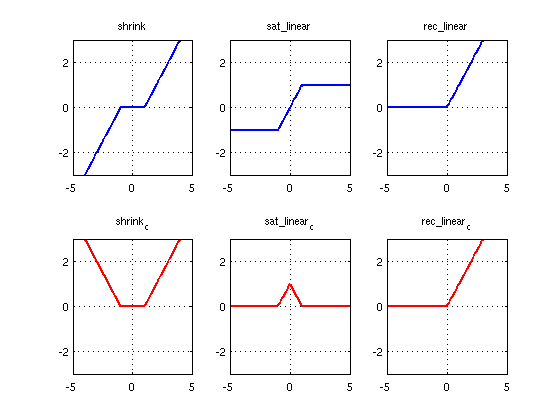
\includegraphics[scale=0.6]{compliments.png}
\caption{Three nonlinearities (top) with their associated complementary functions(bottom).}  
\end{figure} 

\noindent
Figure 1 shows three activation functions and their associated complementary nonlinearities. Let $\theta$ denote all the trainable parameters of the auto-encoder. The complete loss to be minimized by a SATAE with nonlinearity $f$ is: 

\begin{equation} 
L(\theta) = \sum_{x \in D} \frac{1}{2} \|x-x_r\|^2 + \eta \sum_{i=1}^{d_h}f_c(W^e_i x + b^e_i)
\end{equation}    

\noindent
Where $x_r = W^df(W^e x + b^e) + b^d$ is the reconstructed $x$ for an auto-encoder with no output nonlinearity. The hyper-parameter $\eta$ regulates the trade-off between reconstruction and saturation.  

\section{Effect of the Saturation Regularizer} 
We will examine the effect of the saturation regularizer on auto-encoders with a variety of activation functions. It will be shown that the choice of activation function is a significant factor in determining the type of basis the SATAE learns. First, we will present results on toy data in two dimensions followed by results on higher dimensional image data. All of the following results were obtained using stochastic gradient descent.  

\subsection{Visualizing the Energy Landscape}  
Given a trained auto-encoder the reconstruction error can be evaluated for a given input $x$. For low-dimensional spaces ($\mathbb{R}^n$, where $n \leq 3$) we can evaluate the reconstruction error on a regular grid in order to visualize the portions of the space which are well represented by the auto-encoder. More specifically we can compute $E(x) = \frac{1}{2} \|x - x_r \|^2$ for all $x$ within some bounded region of the input space. Ideally, the reconstruction energy will be low for all $x$ which are in training set and high elsewhere. Figure 2 depicts the resulting reconstruction energy for inputs $x \in \mathbb{R}^2$, and  $-1 \leq x_i \leq 1$. Black corresponds to low reconstruction energy. The training data consists of a one dimensional manifold shown overlain in yellow. The auto-encoder contains two encoding basis vectors (red), two decoding basis vectors (green), and uses a saturated-linear activation function. The encoding and decoding bases are unconstrained. The unregularized auto-encoder learns an orthogonal basis with a random orientation. The region of the space which is well reconstructed corresponds to the outer product of the linear regions of two activation functions; beyond that the error increases quadratically with the distance. Including the saturation regularizer however induces the auto-encoder to operate in the saturation regime at the extreme points of the training data, limiting the space which is well reconstructed. Note that because the encoding and decoding weights are separate and unrestricted, the encoding weights were scaled up to effectively reduce the width of the linear regime of the nonlinearity. Figure 3 shows a second toy example for an auto-encoder which uses ten basis vectors and a shrink activation function. Note again that adding the saturation regularizer decreases the volume of the space which is well reconstructed, however good reconstruction is maintained on or near the training data manifold. 

\subsection{SATAE-shrink}
Consider a SATAE with a shrink activation function and shrink parameter $\lambda$. The corresponding complementary nonlinearity, derived using Equation 2 is given by: 
\begin{equation} 
\nonumber
shrink_c(x) =
\begin{cases}
abs(x), \text{ } |x| > \lambda\\
0, \text{ elsewhere}
\end{cases}
\end{equation} 

\begin{figure}
\centering 
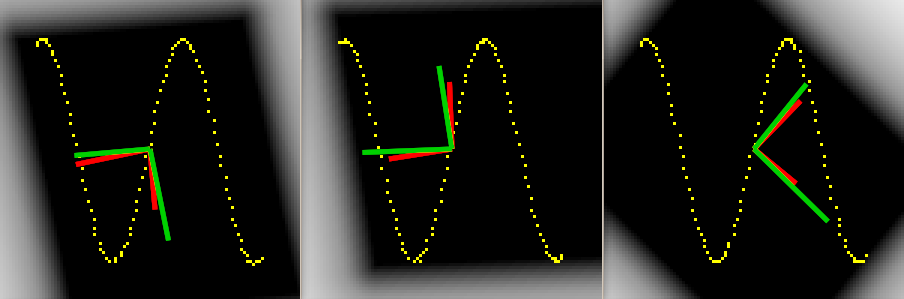
\includegraphics[scale=0.25]{toy_sat_linear_noreg.png}
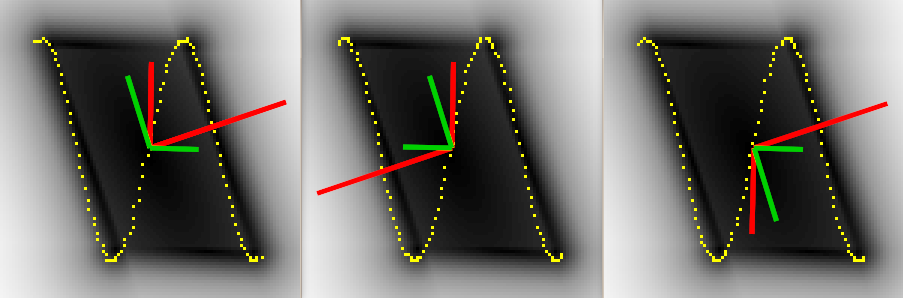
\includegraphics[scale=0.25]{toy_sat_linear_reg.png}
\caption{Three randomly initialized solutions obtained with no regularization (top). Three randomly initialized solutions obtained with regularization (bottom).}  
\end{figure} 

\begin{figure}
\centering 
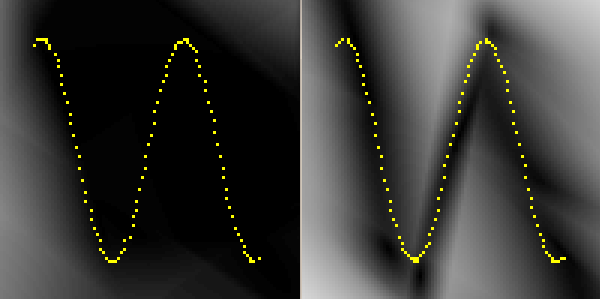
\includegraphics[scale=0.25]{toy_shrink.png}
\caption{Unregularized (left), and regularized (right) solutions obtained using the $shrink$ nonlinearity and 10 basis vectors.}  
\end{figure} 

\noindent
Note that $shrink_c(W^e x + b^e) =  abs(shrink(W^e x + b^e))$, which corresponds to an $L_1$ penalty on the activations. Thus this SATAE is equivalent to a sparse auto-encoder with a shrink activation function. Given the equivalence to the sparse auto-encoder we anticipate the scale ambiguity which occurs with $L_1$ regularization. This ambiguity can be avoided by normalizing the decoder weights to unit norm. It is expected that the SATAE-shrink will learn similar features to those obtain with a sparse auto-encoder, and indeed this is what we observe. Figure 1 shows 25 randomly selected decoder filters (out of 100) learned by an auto-encoder with shrink nonlinearity trained on natural 12x12 image patches. One can recognize the expected Gabor-like features when the saturation penalty is activated and the norm of the decoder filters is constrained to unity. We note that nearly identical results are obtained SATAE which uses a rectified-linear activation function. This is because a rectified-linear function with a bias can behave like as a positive only shrink function, similarly the complementary function is equivalent to a positive only $L_1$ penalty on the activations.          

\begin{figure}
\centering 
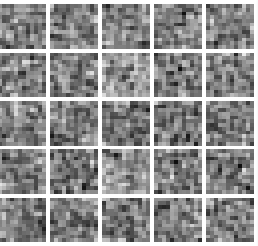
\includegraphics[scale=0.3]{shrink_no_reg.png}
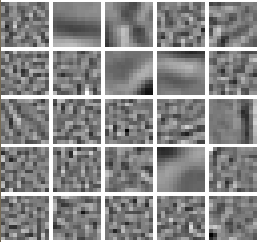
\includegraphics[scale=0.3]{shrink_reg.png}
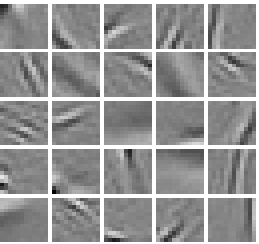
\includegraphics[scale=0.3]{shrink_reg_and_norm.png}
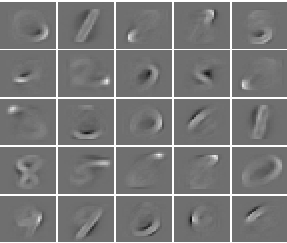
\includegraphics[scale=0.3]{strokes.png}
\caption{Twenty-five out of 100 randomly selected basis elements learned by the auto-encoder with shrink nonlinearity.  (a) No saturation regularization, (b) with saturation regularization , (c) with saturation regularization and constraining the decoder weights to unit norm, (d) identical to (c) but trained on MNIST.}
\end{figure} 

\begin{figure}
\centering 
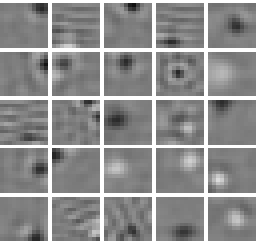
\includegraphics[scale=0.3]{sat_linear_reg2.png}
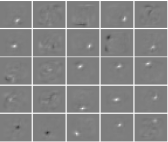
\includegraphics[scale=0.51]{ident.png}
\caption{Twenty-five out of 100 randomly selected basis elements learned by the SATAE with saturated-linear nonlinearity on (a) 12x12 natural image patches, and (b) 28x28 MNIST }
\end{figure} 

\subsection{SATAE-saturated-linear} 
The SATAE with saturated-linear activation function learns a completely different feature set, Empirically, it was observed that increasing the regularization penalty produces more localized feature detectors. To understand why these feature detectors arise consider a dataset in which the variables take on binary values (e.g. MNIST). The scaled identity basis is a global minimum of Equation 3 when a saturated-linear activation function is used. Such a basis can perfectly reconstruct any input while operating exclusively in the saturated regions of the activation function, thus incurring no saturation penalty. This is exactly the type of basis that arises in experiments when training on MNIST, see Figure 5 (b). Training on image patches produces a similar but less pronounced effect, more localized features are obtained but with greater variety. Unlike the SATAE-shrink, the SATAE-saturated-linear receives the heaviest penalty when the activation is zero which tends to spread the responsibility of reconstructing the data among all the basis elements.   

\section{Discussion}
We have demonstrated that drastically different feature sets can be learned by the SATAE by changing the activation function. Our goal is not to advocate the superiority of one features set over another. We merely observe that despite the fact that in all variants the saturation regularizer plays the same role, i.e. the saturation penalty limits the auto-encoder's ability to reconstruct, different results are obtained. This demonstrates that latent state regularizers are not independent of the architecture of the network to which they are applied.   
\end{document} 








